% !TeX spellcheck = fr_FR
\chapter{Sprint 3 – Gestion des PEF}
	
\section*{Introduction}
Dans ce chapitre nous allons principalement nous intéresser à la fonctionnalité la plus  importante de notre projet. Tout comme le sprint précédent, nous procéderons par étapes afin d’éviter d’ignorer une partie de ce sprint.

\section{Backlog sprint}
Dans le backlog du sprint, nous présenterons deux parties suivantes
\subsection{But de sprint}
Le but de ce sprint est de gérer les PEF pour que chaque utilisateur peut les accéder lors l’ouverture de fiche client.
\subsection{User stories}
Après avoir défini l'objectif du sprint, nous pouvons lister les user stories qui appartiennent au sprint.
Le tableau \ref{tab:user-stories-sprint3} liste les différents user stories de notre sprint :
\begin{longtable}[c]{|l|l|l|}
	\hline
	\rowcolor[HTML]{C0C0C0} 
	User stories &
	Tâches &
	complexité \\ \hline
	\endhead
	%
	\begin{tabular}[c]{@{}l@{}}En tant qu’un administrateur, je\\ souhaite de gérer les catégories \\ des PEF\end{tabular} &
	\begin{tabular}[c]{@{}l@{}}Djouter les interfaces de la gestion\\ des catégories des PEF :\\ \tabitem Consultation\\ \tabitem Ajout\\ \tabitem Modification\\ \tabitem Suppression\\ \tabitem Recherche\\ et la logique derrière\end{tabular} &
	2 \\ \hline
	\begin{tabular}[c]{@{}l@{}}En tant qu’un administrateur, je\\ souhaite de gérer les types\\ des catégories des PEF\end{tabular} &
	\begin{tabular}[c]{@{}l@{}}Ajouter les interfaces de la gestion\\ des types de catégories :\\ \tabitem Consultation\\ \tabitem Ajout\\ \tabitem Modification\\ \tabitem Suppression\\ \tabitem Recherche\\ et la logique derrière\end{tabular} &
	2 \\ \hline
	\begin{tabular}[c]{@{}l@{}}En tant qu’un administrateur, je\\ souhaite de gérer les PEF\end{tabular} &
	\begin{tabular}[c]{@{}l@{}}Ajouter les interfaces de la gestion\\ des PEF :\\ \tabitem Consultation\\ \tabitem Ajout\\ \tabitem Modification\\ \tabitem Suppression\\ \tabitem Recherche\\ et la logique derrière\end{tabular} &
	2 \\ \hline
	\begin{tabular}[c]{@{}l@{}}En tant qu’un administrateur, je\\ souhaite de consulter les types \\ des PEF\end{tabular} &
	\begin{tabular}[c]{@{}l@{}}Ajouter les interfaces de consultation \\ des types des PEF :\\ \tabitem Consultation \\ \tabitem Recherche\\ et la logique derrière\end{tabular} &
	3 \\ \hline
	\begin{tabular}[c]{@{}l@{}}En tant qu’un administrateur, je\\ souhaite de gérer la visibilité \\ des PEF au boutique\end{tabular} &
	\begin{tabular}[c]{@{}l@{}}Ajouter les interfaces de la gestion\\ de visibilité des PEF :\\ \tabitem Consultation\\ \tabitem Ajout\\ \tabitem Modification\\ \tabitem Suppression\\ \tabitem Recherche\\ et la logique derrière\end{tabular} &
	1 \\ \hline
	\begin{tabular}[c]{@{}l@{}}En tant qu’un conseiller client réactif, je\\ souhaite de consulter les PEF \\ disponibles lors l’ouverture de\\ fiche client\end{tabular} &
	\begin{tabular}[c]{@{}l@{}}Fournir la liste des PEF au \\ conseiller client réactif en fonction \\ de type de l’utilisateur ( CPRO \\ pour boutique ou 3901 pour \\ centre d’appel) de catégorie et de\\  type de catégorie\end{tabular} &
	1 \\ \hline
	\begin{tabular}[c]{@{}l@{}}En tant qu’un administrateur, je\\ souhaite d’avoir une vue totale \\ des logs des APIs\end{tabular} &
	\begin{tabular}[c]{@{}l@{}}Développer une interface qui \\ comporte les informations \\ complètes de logs APIs\end{tabular} &
	2 \\ \hline
	\begin{tabular}[c]{@{}l@{}}En tant qu’un administrateur, je\\ souhaite de tracer toutes actions\\ prises par les utilisateurs sur\\ l’application\end{tabular} &
	\begin{tabular}[c]{@{}l@{}}Elaborer les logs de navigation sur \\ l’application et les actions prises\end{tabular} &
	3 \\ \hline
	\captionsetup{justification=centering}
	\caption{User stories de sprint 3}
	\label{tab:user-stories-sprint3}\\
\end{longtable}

\section{Etude de réalisation du sprint 3}
Cette section de notre projet présente les différents diagrammes de cas d’utilisation avec leurs raffinements.
\subsection{Diagramme de cas d’utilisation global sprint 3}
La figure \ref{fig:usecase-sprint3} décrit le diagramme de cas d’utilisation global du sprint 3.
\begin{figure}[H]
	\centering
	\includegraphics[width=0.58\linewidth]{"img/conception/usecases/sprint 3/UseCase-sprint3"}
	\caption[Diagramme de cas d’utilisation global sprint 3]{Diagramme de cas d’utilisation global sprint 3}
	\label{fig:usecase-sprint3}
\end{figure}

\subsection{Raffinement et description textuelle des diagrammes de cas d’utilisation}
Dans cette section, nous présentons les diagrammes des cas d’utilisation détaillés et leurs descriptions textuelles.\newpage
\subsubsection{Cas d’utilisation «gestion des catégories»}
La figure \ref{fig:usecase-gestion-categories} illustre le raffinement du cas d’utilisation « gestion des catégories »

\begin{figure}[H]
	\centering
	\includegraphics[width=0.7\linewidth]{"img/conception/usecases/sprint 3/usecase-gestion-categories"}
	\caption[Cas d’utilisation «gestion des catégories»]{Gas d’utilisation «gestion des catégories»}
	\label{fig:usecase-gestion-categories}
\end{figure}

\myparagraph{Description textuelle du cas d’utilisation «gestion des catégories»}
Le tableau \ref{tab:descrip-text-gestion-cat} contient la description textuelle du cas d’utilisation «gestion des catégories»
\begin{table}[H]
	\centering
	\begin{tabular}{|l|l|}
		\hline
		\rowcolor[HTML]{C0C0C0} 
		Cas d’utilisation & Gestion des catégories                     \\ \hline
		Acteur            & Administrateur                             \\ \hline
		Résumé            & L’administrateur peut gérer les catégories \\ \hline
		Précondition      & L’administrateur doit être authentifié     \\ \hline
		Scénario principal &
		\begin{tabular}[c]{@{}l@{}}Pour gérer les catégories, l’administrateur peut :\\ Ajouter une catégorie\\ Modifier une catégorie ou les types d'une catégorie\\ Supprimer une catégorie\\ Consulter les catégories\\ Rechercher des catégories\end{tabular} \\ \hline
		Post condition    & Mettre à jour la liste des catégories      \\ \hline
	\end{tabular}
	\captionsetup{justification=centering}
	\caption{Description textuelle du cas d’utilisation «gestion des catégories»}
	\label{tab:descrip-text-gestion-cat}
\end{table}
\subsubsection{Cas d’utilisation «gestion des PEF»}
La figure \ref{fig:usecase-gestion-pef} illustre le raffinement du cas d’utilisation «gestion des PEF»
\begin{figure}[H]
	\centering
	\includegraphics[width=1\linewidth]{"img/conception/usecases/sprint 3/usecase-gestion-PEF"}
	\caption[Cas d’utilisation «gestion des PEF»]{Cas d’utilisation «gestion des PEF»}
	\label{fig:usecase-gestion-pef}
\end{figure}
\newpage
\myparagraph{Description textuelle du cas d’utilisation «gestion des PEF»}
Le tableau \ref{tab:descrip-text-gestion-pef} contient la description textuelle du ccas d’utilisation «gestion des PEF».
\begin{table}[H]
	\centering
	\begin{tabular}{|l|l|}
		\hline
		\rowcolor[HTML]{C0C0C0} 
		Cas d’utilisation & Gestion des PEF                        \\ \hline
		Acteur            & Administrateur                         \\ \hline
		Résumé            & L’administrateur peut gérer les PEF    \\ \hline
		Précondition      & L’administrateur doit être authentifié \\ \hline
		Scénario principal &
		\begin{tabular}[c]{@{}l@{}}Pour gérer les PEF , l’administrateur peut :\\ Ajouter un PEF \\ Modifier un PEF \\ Supprimer un PEF \\ Consulter les PEF \\ Rechercher des PEF\end{tabular} \\ \hline
		Post condition    & Mettre à jour la liste des PEF         \\ \hline
	\end{tabular}
\captionsetup{justification=centering}
	\caption{Description textuelle du cas d’utilisation «gestion des PEF»}
	\label{tab:descrip-text-gestion-pef}
\end{table}

\subsubsection{Cas d’utilisation «visibilité des PEF au boutique»}
La figure \ref{fig:usecase-gestion-visibilite} illustre le raffinement du cas d’utilisation «gestion des PEF»

\begin{figure}[H]
	\centering
	\includegraphics[width=1\linewidth]{"img/conception/usecases/sprint 3/usecase-gestion-visibilite"}
	\caption[Cas d’utilisation «visibilité des PEF au boutique»]{Cas d’utilisation «visibilité des PEF au boutique»}
	\label{fig:usecase-gestion-visibilite}
\end{figure}

\myparagraph{Description textuelle du cas d’utilisation «visibilité des PEF au boutique»}
Le tableau \ref{tab:descrip-text-visib} contient la description textuelle du cas d’utilisation «visibilité des PEF au boutique»

\begin{table}[H]
	\centering
	\begin{tabular}{|l|l|}
		\hline
		\rowcolor[HTML]{C0C0C0} 
		Cas d’utilisation & Visibilité des PEF au boutique                                                  \\ \hline
		Acteur            & Administrateur                                                                  \\ \hline
		Résumé            & L’administrateur peut donner l’autorité à une boutique pour utiliser un tel PEF \\ \hline
		Précondition &
		\begin{tabular}[c]{@{}l@{}}l’administrateur doit être authentifié\\ La boutique doit être existante\\ Le PEF doit être existant\end{tabular} \\ \hline
		Scénario principal &
		\begin{tabular}[c]{@{}l@{}}Pour gérer la visibilité , l’administrateur peut :\\ ajouter un PEF à une boutique\\ Modifier la visibilité de boutique\\ limiter la visibilité de boutique\\ Consulter les visibilités des boutiques\\ Rechercher des visibilités boutiques\end{tabular} \\ \hline
		Post condition    & Mettre à jour la liste des visibilités                                          \\ \hline
	\end{tabular}
	\captionsetup{justification=centering}
	\caption{Description textuelle du cas d’utilisation «visibilité des PEF au boutique»}
	\label{tab:descrip-text-visib}
\end{table}

\subsubsection{Description textuelle du cas d’utilisation «consultation fiche client»}
Le tableau \ref{tab:descrip-text-fiche-client} contient la description textuelle du cas d’utilisation «consultation fiche client»
\begin{table}[H]
	\centering
	\begin{tabular}{|l|l|}
		\hline
		\rowcolor[HTML]{C0C0C0} 
		Cas d’utilisation & Consultation fiche client                                                                        \\ \hline
		Acteur            & Le conseiller client réactif et l’administrateur                                                 \\ \hline
		Résumé &
		\begin{tabular}[c]{@{}l@{}}Les acteurs auront une liste des PEF classés selon\\ leur catégorie en fonction de type d’utilisateur, type\\ des catégories\end{tabular} \\ \hline
		Précondition      & \begin{tabular}[c]{@{}l@{}}L’acteur doit être authentifié\\ Ouvrir une fiche client\end{tabular} \\ \hline
		Scénario principal &
		\begin{tabular}[c]{@{}l@{}}Pour consulter les PEF, l’acteur doit ouvrir\\ une fiche client. Puis un menu sera affiché\\ contenant la liste des applications.\\ Cette dernière contient les PEF classés selon\\ leurs catégories.\end{tabular} \\ \hline
	\end{tabular}
	\captionsetup{justification=centering}
	\caption{Description textuelle du cas d’utilisation «consultation fiche client»}
	\label{tab:descrip-text-fiche-client}
\end{table}

\subsubsection{Description textuelle du cas d’utilisation «consultation des logs API»}
Le tableau \ref{tab:descrip-text-api-logs} contient la description textuelle du cas d’utilisation «consultation des logs API»

\begin{table}[H]
	\centering
	\begin{tabular}{|l|l|}
		\hline
		\rowcolor[HTML]{C0C0C0} 
		Cas d’utilisation & consultation des logs API                                                                                                 \\ \hline
		Acteur            & administrateur                                                                                                            \\ \hline
		Résumé            & L’administrateur peut consulter les logs des APIs                                                                         \\ \hline
		précondition      & \begin{tabular}[c]{@{}l@{}}l’administrateur doit être authentifié\\ Les fichiers logs doivent être existants\end{tabular} \\ \hline
		scénario principal &
		\begin{tabular}[c]{@{}l@{}}Pour consultation des logs API , l’administrateur\\ va consulter le tableau des statistiques des logs.\\ Si l’administrateur souhaite d’avoir des informations\\ détaillées, il peut cliquer sur la colonne de table \\ et un modal sera affiché contenant toutes les détails\end{tabular} \\ \hline
	\end{tabular}
	\captionsetup{justification=centering}
	\caption{Description textuelle du cas d’utilisation «consultation des logs API»}
	\label{tab:descrip-text-api-logs}
\end{table}

\subsubsection{Description textuelle du cas d’utilisation «élaboration des logs Panoramix»}
Le tableau \ref{tab:descrip-text-elab-logs} contient la description textuelle du cas d’utilisation «élaboration des logs Panoramix»

\begin{longtable}[c]{|l|l|}
	\hline
	\rowcolor[HTML]{C0C0C0} 
	Cas d’utilisation & Elaboration des logs Panoramix                                                                                                                         \\ \hline
	\endfirsthead
	%
	\endhead
	%
	Acteur            & Système                                                                                                                                                \\ \hline
	Résumé            & \begin{tabular}[c]{@{}l@{}}Après chaque action prise par les utilisateurs,\\ le système doit écrire dans le log cette action\\ en détails\end{tabular} \\ \hline
	Précondition      & Une action est prise par un utilisateur                                                                                                                \\ \hline
	Scénario principal &
	\begin{tabular}[c]{@{}l@{}}Chaque navigation ou action prise sur Panoramix,\\ le système doit décrire cette action sous un tel\\ format  structuré qui comporte\\ les informations suivante :\\ \tabitem Date d’action\\ \tabitem Heure d’action\\ \tabitem CUID d’utilisateur\\ \tabitem Nom d’utilisateur\\ \tabitem Prénom de l’utilisateur\\ \tabitem Sujet d’action\\ \tabitem L’action\\ \tabitem Etat d’action\\ \tabitem Rôle d’utilisateur\\ \tabitem Département d’utilisateur \\ \tabitem etc..\\ Ces champs doivent être séparés par une “;”\end{tabular} \\ \hline
	Post condition    & Le fichier log sera rédigé                                                                                                                             \\ \hline
	\caption{Description textuelle du cas d’utilisation «élaboration des logs Panoramix»}
	\label{tab:descrip-text-elab-logs}\\
\end{longtable}

\section{Conception}
Dans cette partie, nous présentons les différents diagrammes de classes ainsi que de séquence détaillés pour ce sprint. 


\subsection{Diagramme de classes}
la figure \ref{fig:classdiag-sprint3} illustre la structure statique du sprint 3 schématisé dans un diagramme de classe globale.
Dans ce sprint, nous ajoutons les dernières 3 classes :
\begin{itemize}
	\item \textbf{La classe Categorie :} représente les catégories des PEF. Ces catégories peuvent avoir un ou plusieurs types.
	\item \textbf{La classe Application :} représente les applications et leurs URL d'accès. Chaque application est composée par des PEF.
	\item \textbf{La classe PEF :} représente les PEF à utilisés. Ces PEF peut appartenir à une ou plusieurs boutique autrement cette boutique peut l'utiliser. Ainsi que, les PEF doivent avoir une ou plusieurs catégories. 
\end{itemize}
\begin{figure}[H]
	\centering
	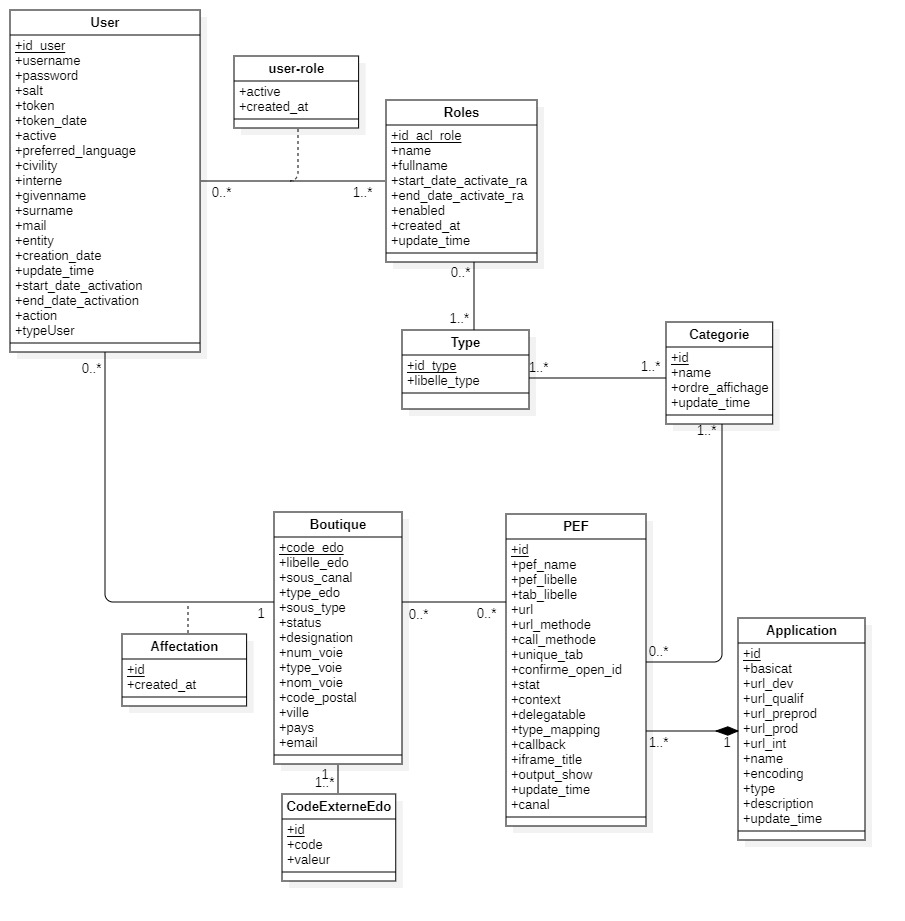
\includegraphics[width=1\linewidth]{img/conception/classes/ClassDiag-sprint3}
	\caption[Diagramme de classes sprint 3]{Diagramme de classes sprint 3}
	\label{fig:classdiag-sprint3}
\end{figure}

\subsection{Diagrammes de séquences détaillés}
Nous allons maintenant passer à l’aspect dynamique des opérations représentées dans le diagramme de classe à l’aide des diagrammes de séquences de système et d’objets.
\subsubsection{Quelques diagramme de séquences système de Sprint 3}
Dans cette section, nous présenterons quelques diagrammes de séquences système de «gestion des PEF» tels que : \newpage

\myparagraph{Diagramme de séquences système de «visibilité des PEF au boutique»} 
Après la consultation de page de visibilité, l'administrateur remplit la formulaire par le nom du PEF et le nom de la boutique puis il valide. Le système vérifie l'existence du PEF et la boutique et insère les données.\\
Un message de succès ou d'échec sera affiché.
	\begin{figure}[H]
		\centering
		\includegraphics[width=0.7\linewidth]{"img/conception/sequences/sprint 3/visibilite-system"}
		\caption[Diagramme de séquences système de «visibilité des PEF au boutique»]{Diagramme de séquences système de «visibilité des PEF au boutique»}
		\label{fig:visibilite-system}
	\end{figure}


\subsubsection{Quelques diagramme de séquences objets de Sprint 3}
Nous présentons dans ce qui suit quelques diagrammes de séquences objets détaillés \\du sprint 3.
\myparagraph{Diagramme de séquences d’objets de «consultation logs API»} 
Lors la consultation des logs API, le contrôleur de consultation va parcourir tous les fichiers logs et les transformer en format JSON. Ces informations seront représentées sous format de tableau dans l'IHM. 
	\begin{figure}[H]
		\centering
		\includegraphics[width=0.7\linewidth]{"img/conception/sequences/sprint 3/log-api-obj"}
		\caption[Diagramme de séquences d’objets de «consultation logs API»]{Diagramme de séquences d’objets de «consultation logs API»}
		\label{fig:log-api-obj}
	\end{figure}
	\newpage
\myparagraph{Diagramme de séquences d’objets de «fiche client»} 
Après la choix de client, une liste des PEF doit être affichée. Ces PEF seront filtrés en fonction de type d'utilisateur, autrement un conseiller client réactif de boutique n'utilise que des PEF de catégorie ayant le type CPRO. 
	\begin{figure}[H]
		\centering
		\includegraphics[width=0.7\linewidth]{"img/conception/sequences/sprint 3/fiche-client-obj"}
		\caption[Diagramme de séquences d’objets de «fiche client»]{Diagramme de séquences d’objets de «fiche client»}
		\label{fig:fiche-client-obj}
	\end{figure}

\section{Réalisation}
Dans cette section, nous allons exposer les différentes interfaces réalisées dans le sprint 3.
\subsection{Interfaces de gestion des catégories}
\begin{itemize}
	\item Consultation des catégories et recherche
	\begin{figure}[H]
		\centering
		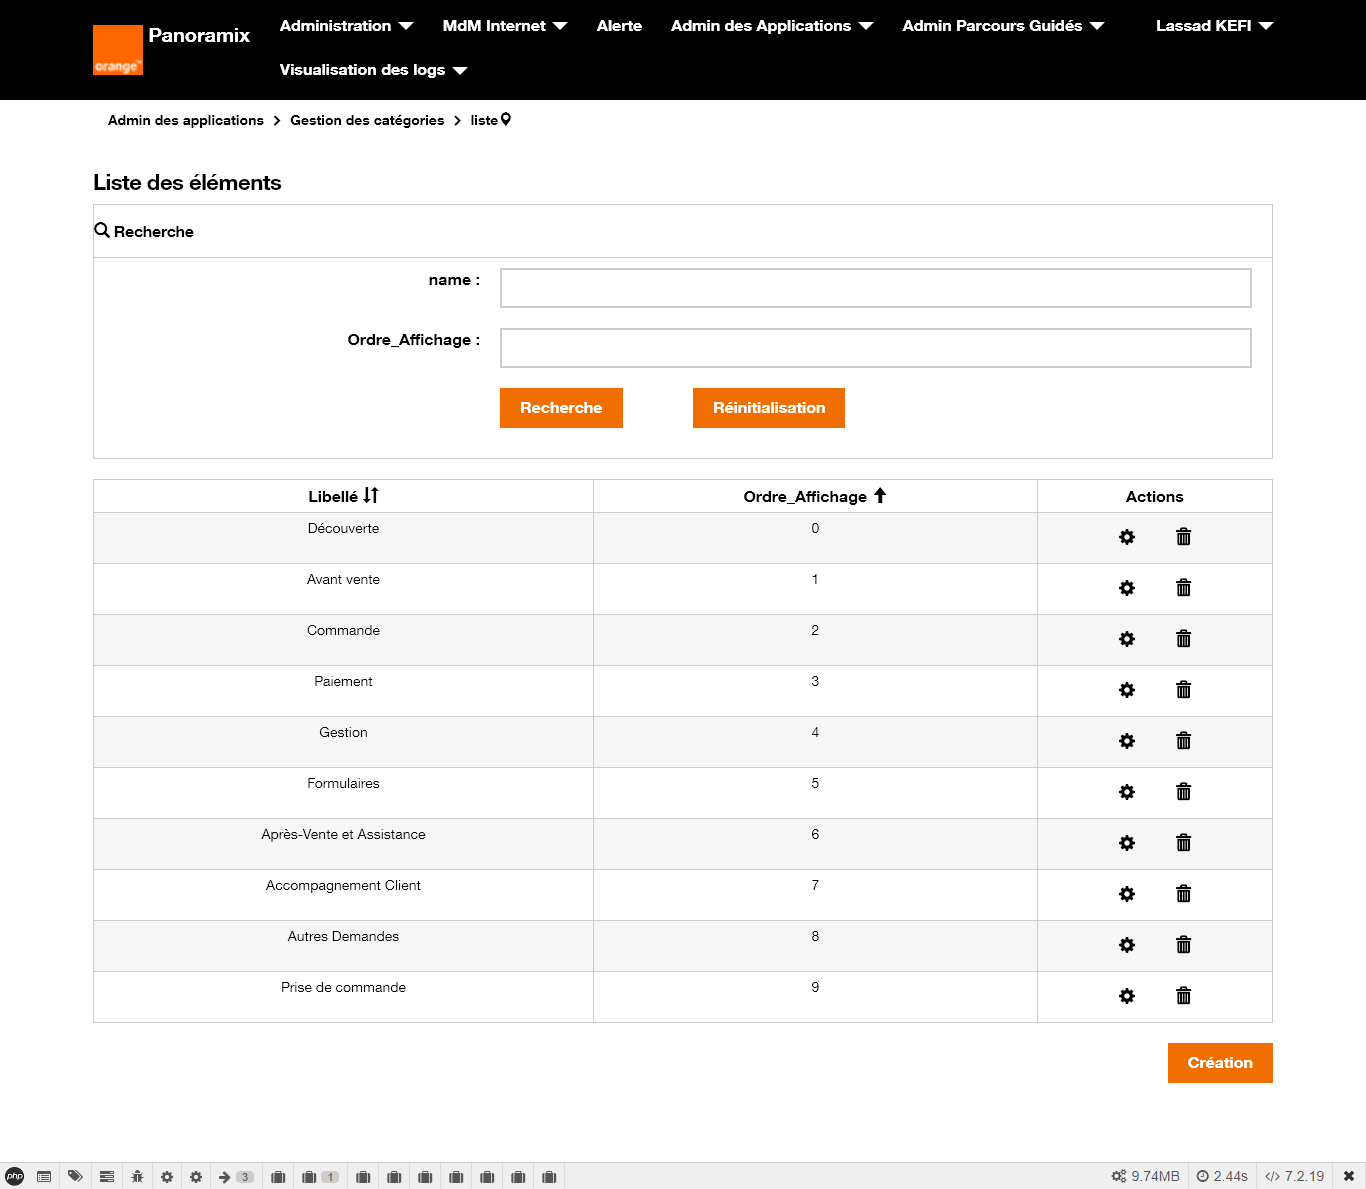
\includegraphics[width=0.5\linewidth]{img/screenshots/categorie/index}
		\caption[Interface consultation des catégories et recherche]{Interface consultation des catégories et recherche}
		\label{fig:index-categorie}
	\end{figure}
	\newpage
	\item Modifier ou créer une catégories
	\begin{figure}[H]
		\centering
		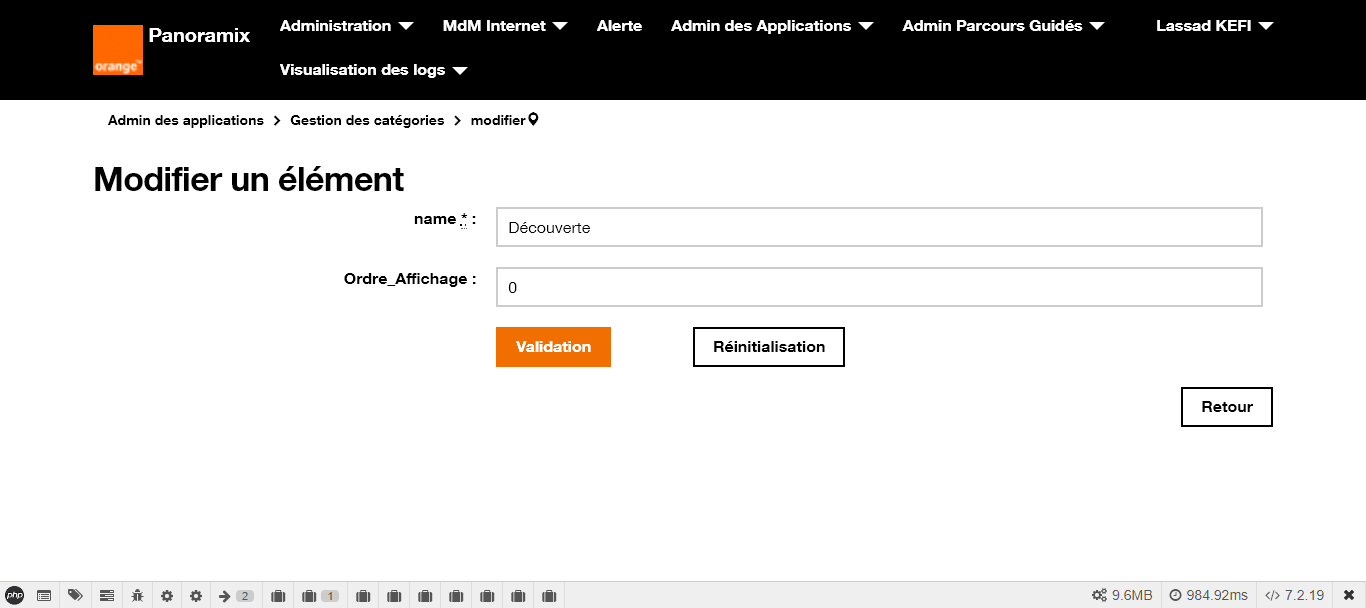
\includegraphics[width=0.6\linewidth]{img/screenshots/categorie/create-edit}
		\caption[Interface modifier une catégorie]{Interface modifier une catégorie}
		\label{fig:edit-categorie}
	\end{figure}

	\item Supprimer une catégories
	\begin{figure}[H]
		\centering
		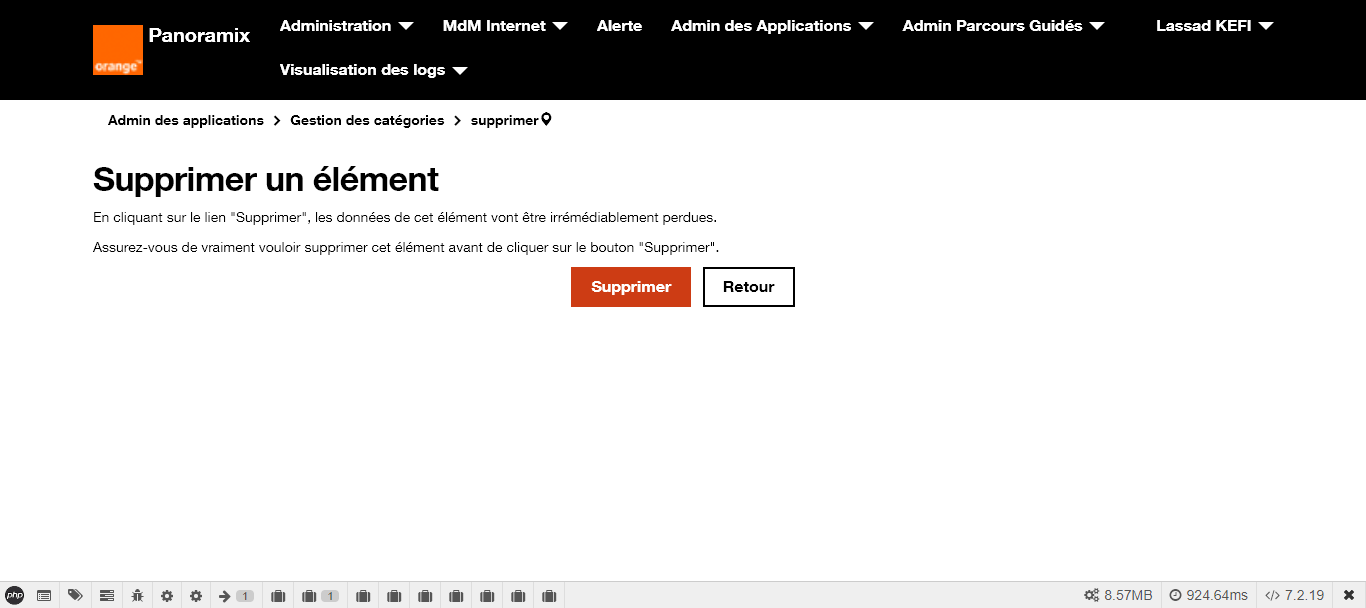
\includegraphics[width=0.6\linewidth]{img/screenshots/categorie/delete}
		\caption[Interface supprimer une catégorie]{Interface supprimer une catégorie}
		\label{fig:delete-categorie}
	\end{figure}
\end{itemize}

\subsection{Interfaces de gestion des type de catégories}

\begin{itemize}
	\item Consultation des types des catégories
	\begin{figure}[H]
		\centering
		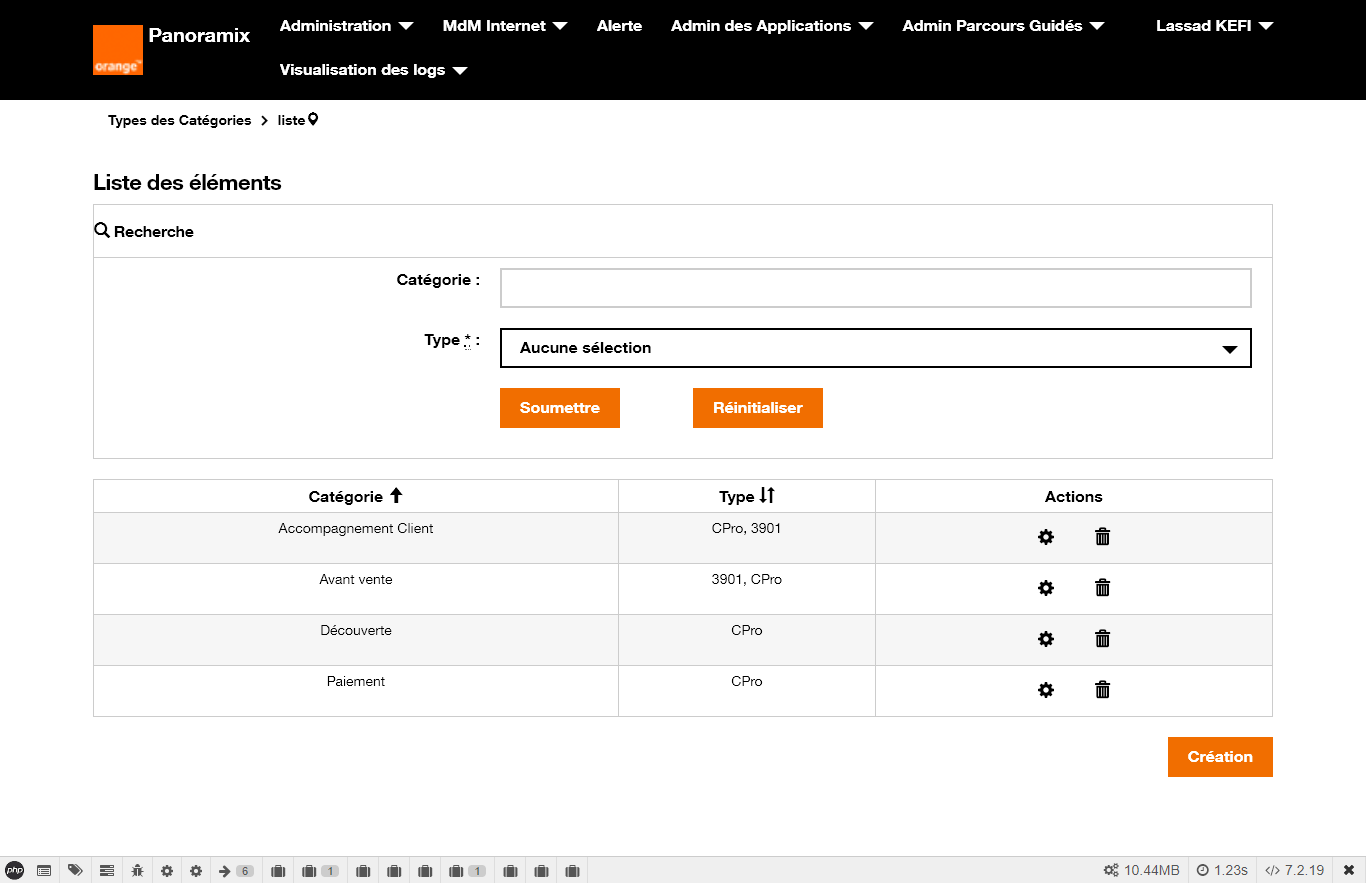
\includegraphics[width=0.6\linewidth]{img/screenshots/categorie-type/index}
		\caption[Interface consultation des types des catégories]{Interface consultation des types des catégories}
		\label{fig:index-tc}
	\end{figure}
	\newpage
	\item Voir un type des catégories
	\begin{figure}[H]
		\centering
		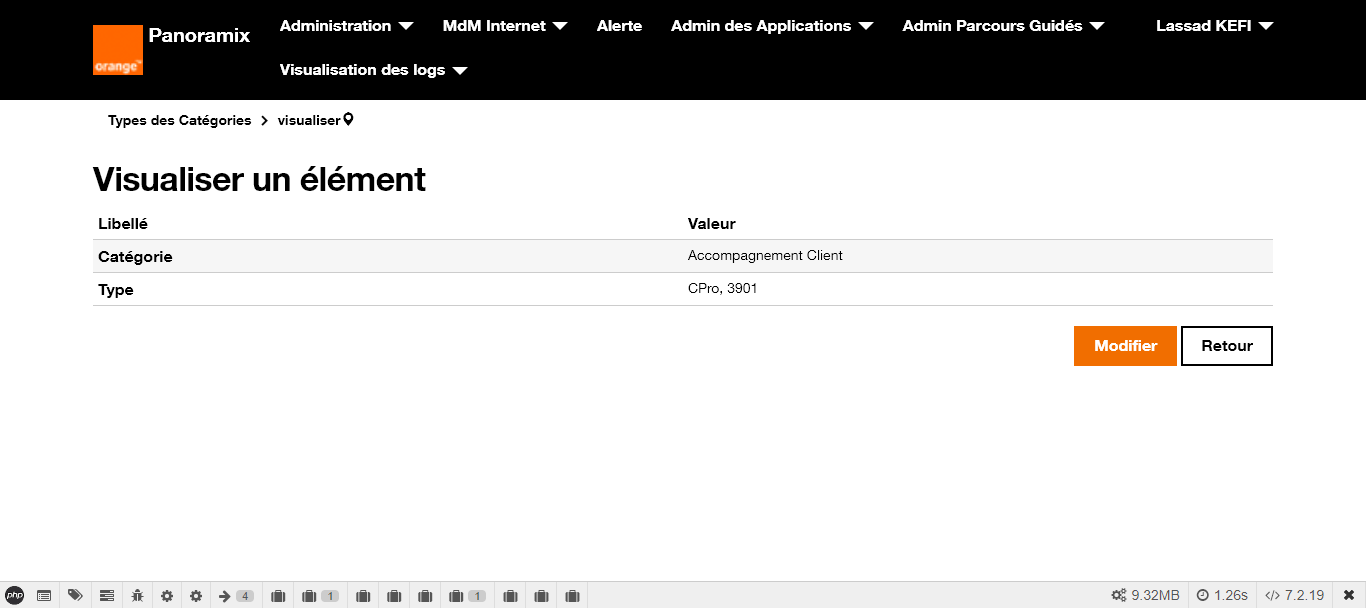
\includegraphics[width=0.7\linewidth]{img/screenshots/categorie-type/view}
		\caption[Interface voir un type des catégories]{Interface voir un type des catégories}
		\label{fig:view-tc}
	\end{figure}
	
	\item Modifier ou créer un type des catégories
	\begin{figure}[H]
		\centering
		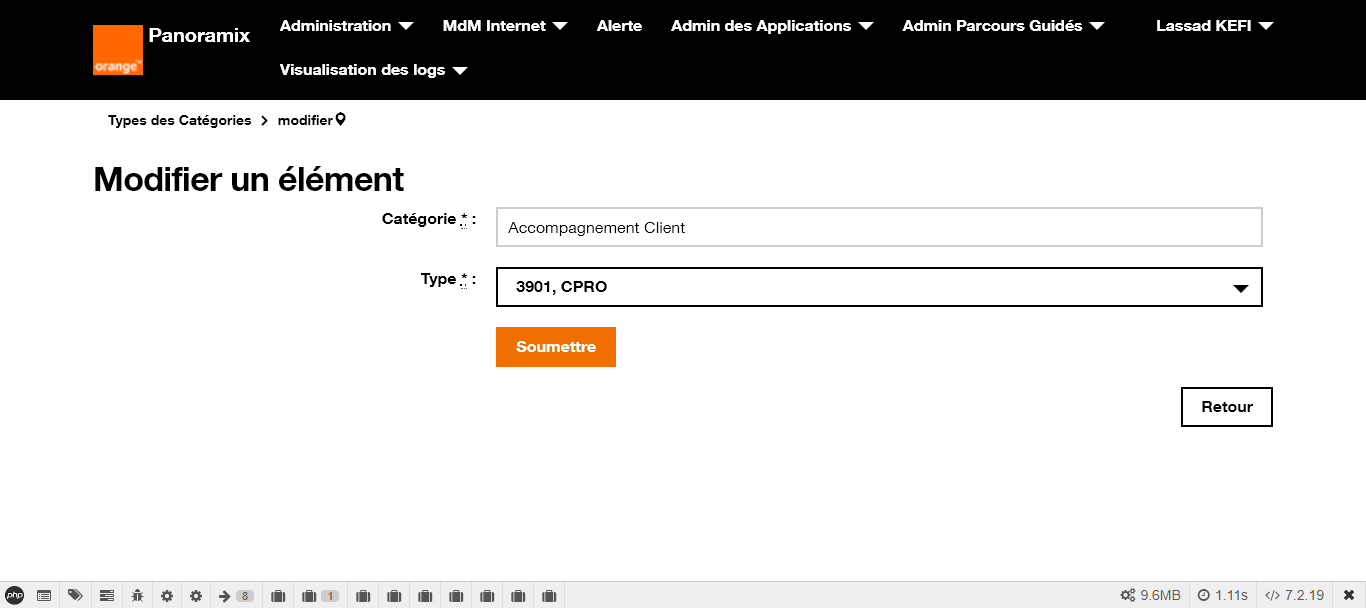
\includegraphics[width=0.7\linewidth]{img/screenshots/categorie-type/create-edit}
		\caption[Interface modifier un type des catégories]{Interface modifier un type des catégories}
		\label{fig:edit-tc}
	\end{figure}

	\item Supprimer un type des catégories
	\begin{figure}[H]
		\centering
		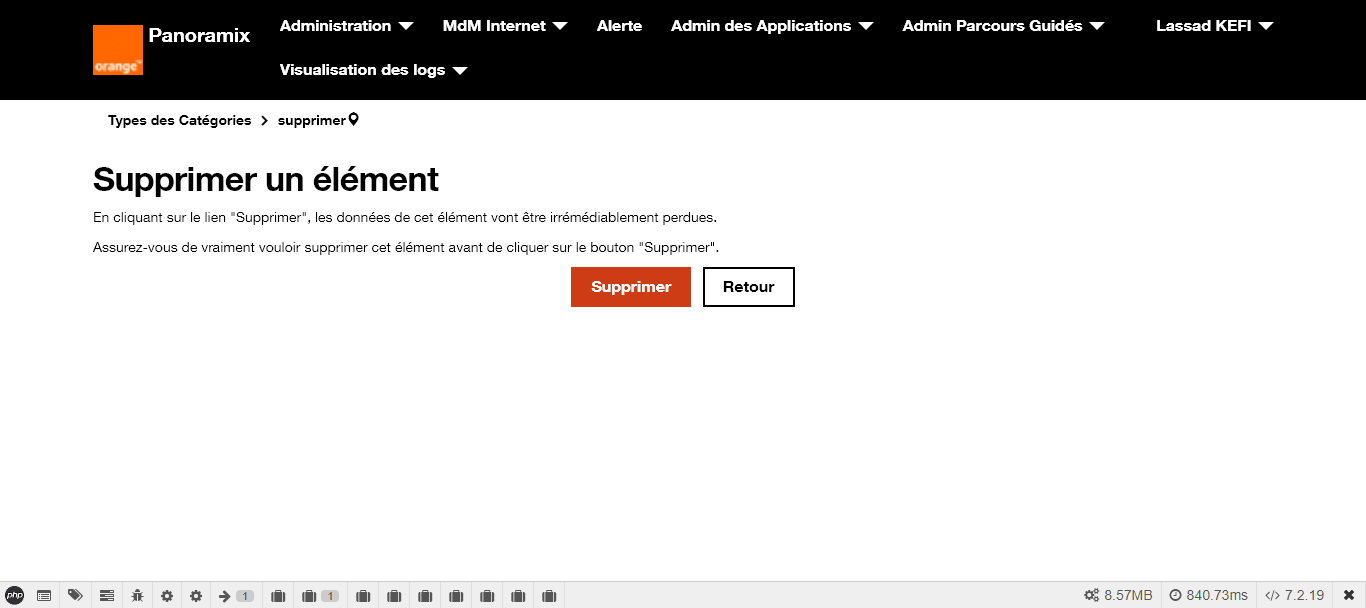
\includegraphics[width=0.7\linewidth]{img/screenshots/categorie-type/delete}
		\caption[Interface supprimer un type des catégories]{Interface supprimer un type des catégories}
		\label{fig:delete-tc}
	\end{figure}
\end{itemize}
\newpage
\subsection{Interfaces de gestion des PEF}
\begin{itemize}
	\item Consultation des PEF et recherche
	\begin{figure}[H]
		\centering
		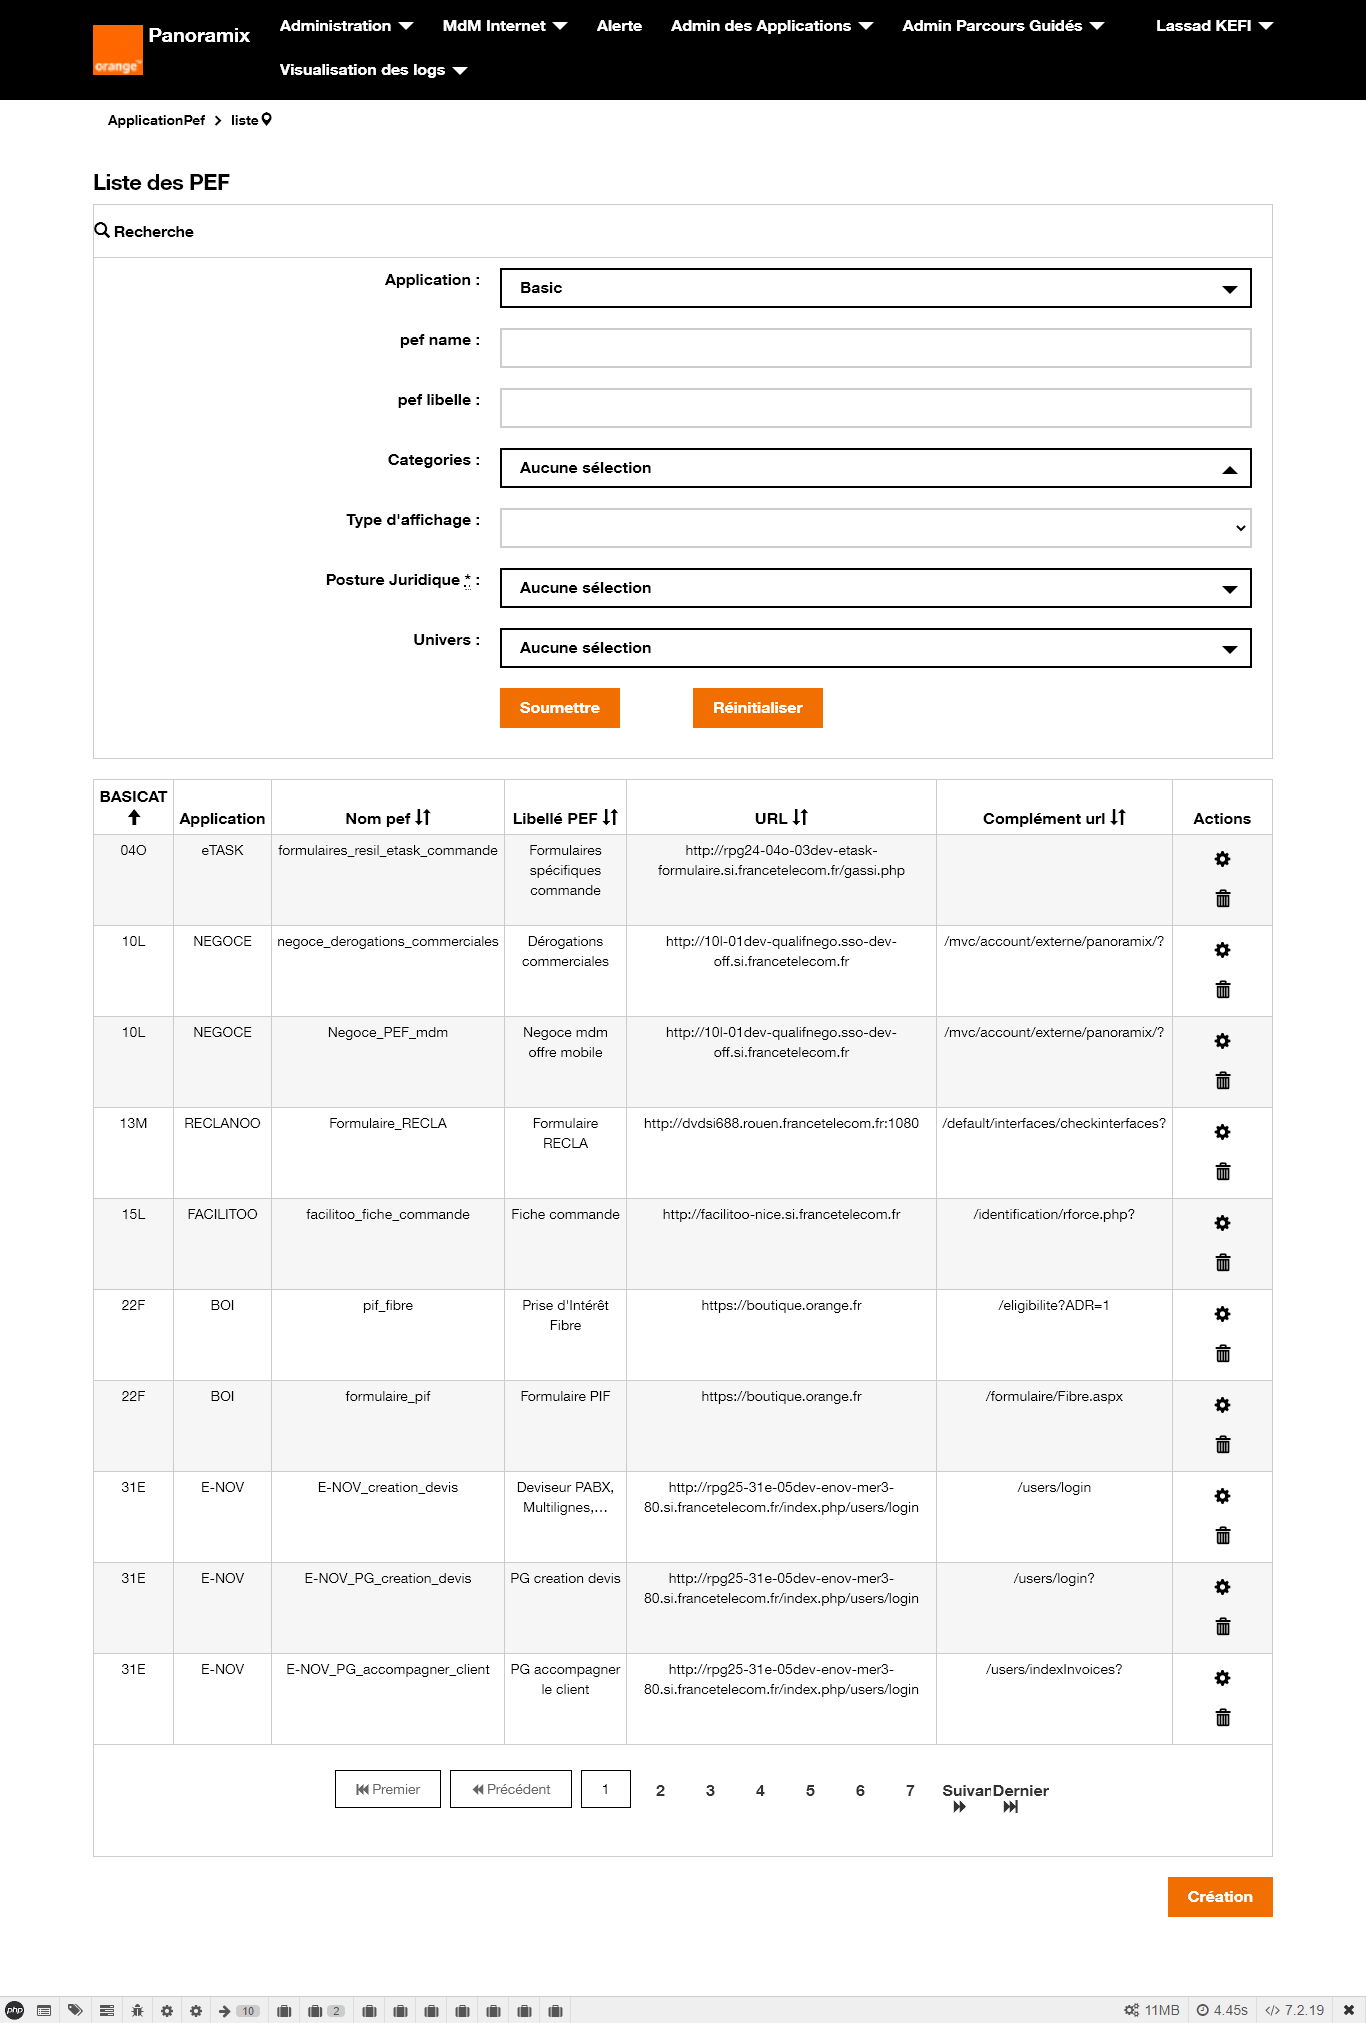
\includegraphics[width=0.55\linewidth]{img/screenshots/pef/index}
		\caption[Interface consultation des PEF et recherche]{Interface consultation des PEF et recherche}
		\label{fig:index-pef}
	\end{figure}

	\item Voir les données d'un PEF
	\begin{figure}[H]
		\centering
		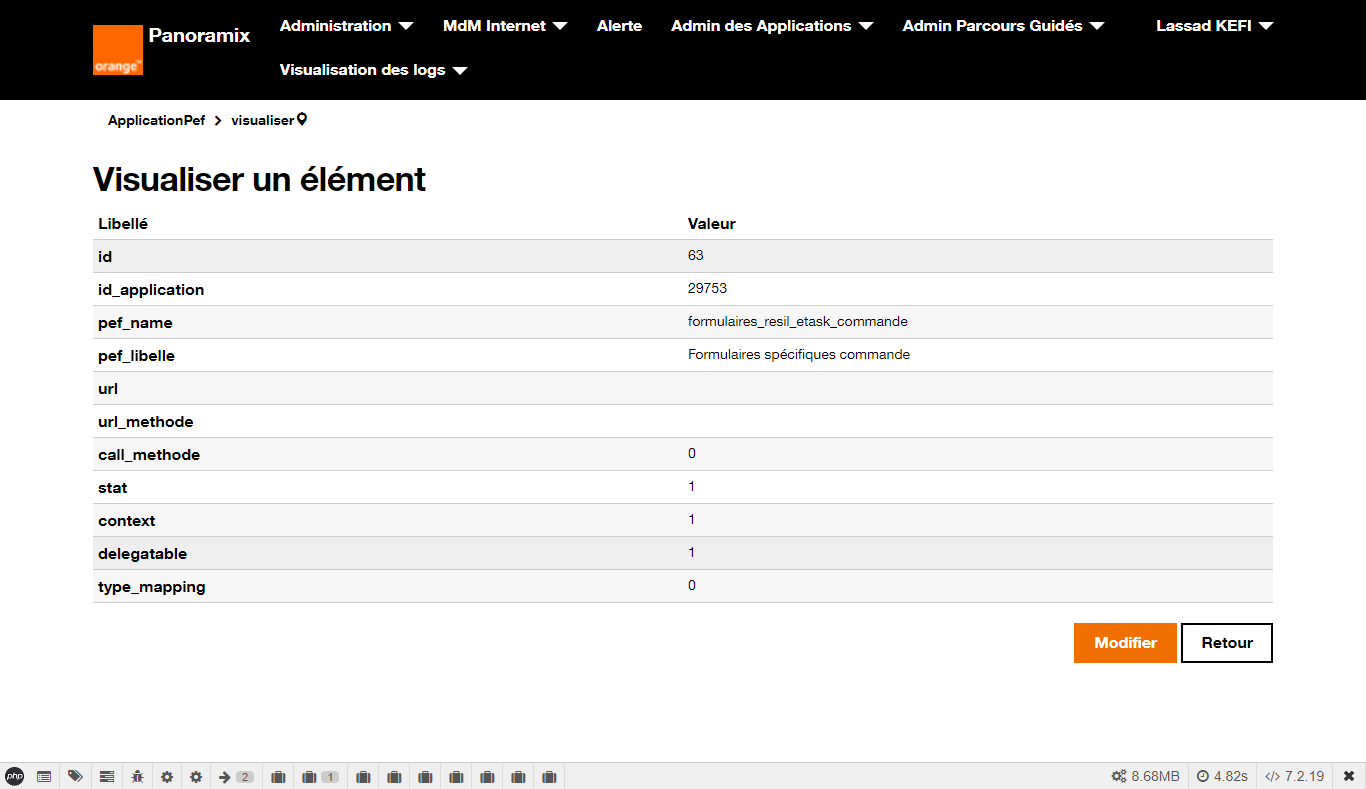
\includegraphics[width=0.55\linewidth]{img/screenshots/pef/view}
		\caption[Interface voir les données d'un PEF]{Interface voir les données d'un PEF}
		\label{fig:view-pef}
	\end{figure}
	\newpage
	\item Modifier ou créer un PEF
	\begin{figure}[H]
		\centering
		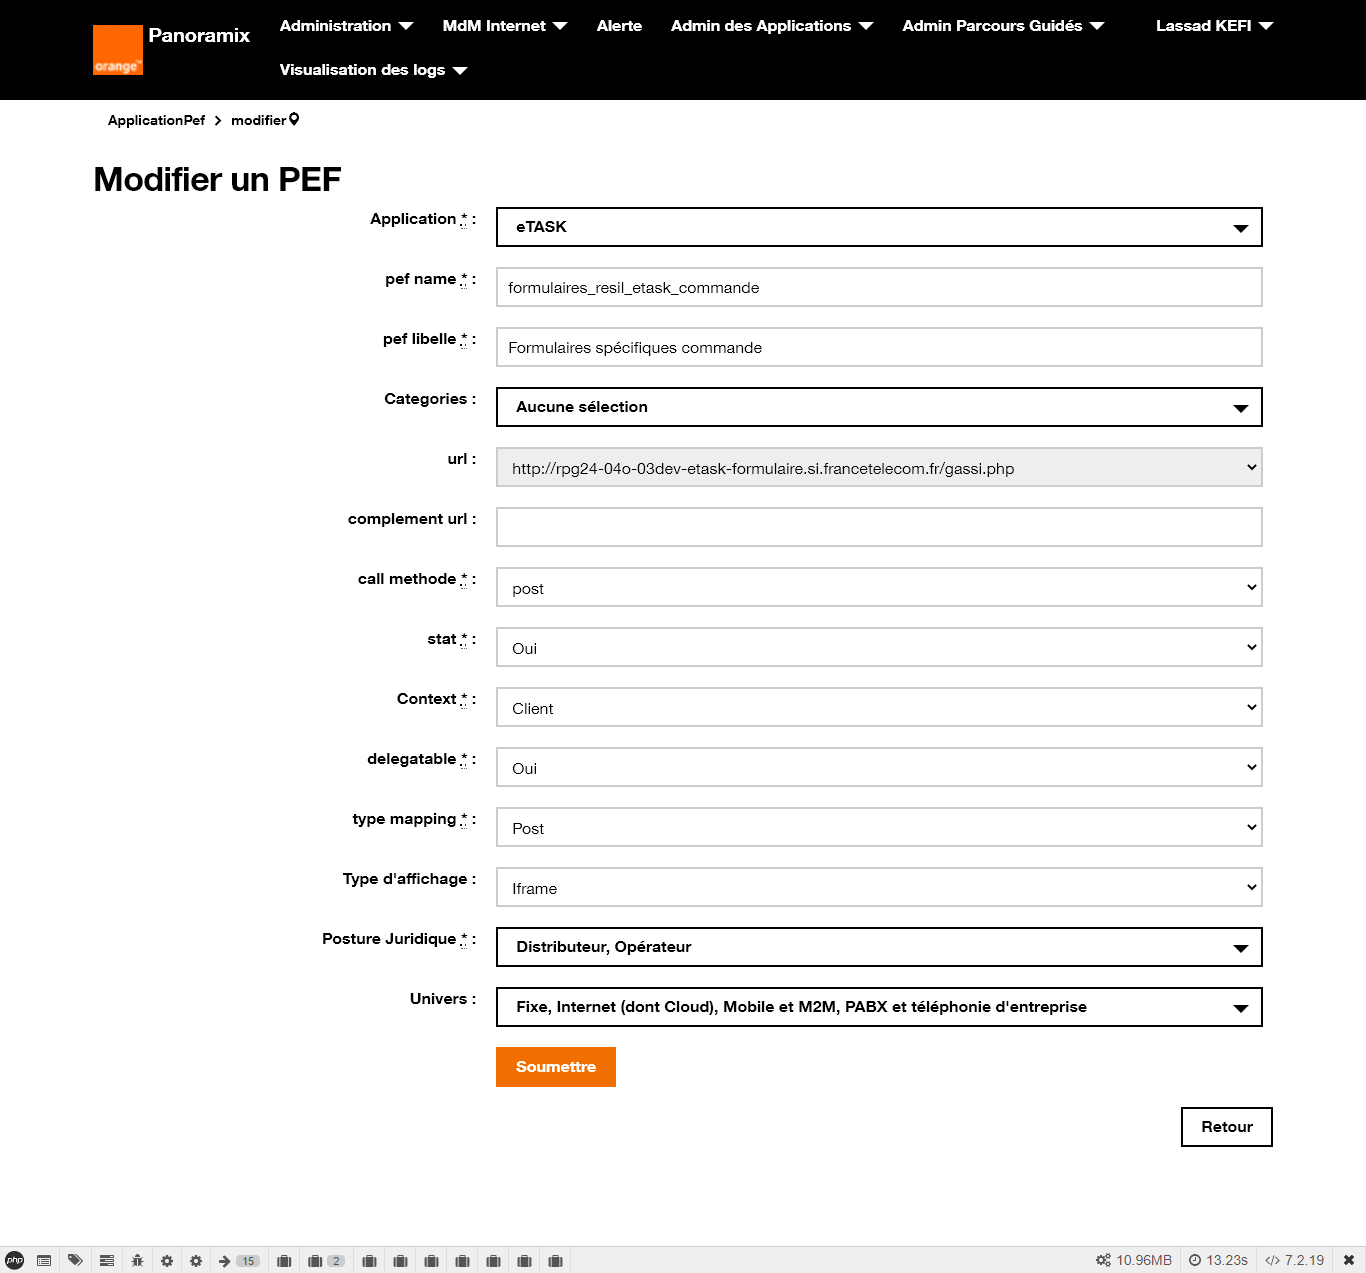
\includegraphics[width=0.7\linewidth]{img/screenshots/pef/edit}
		\caption[Interface modifier ou créer un PEF]{Interface modifier ou créer un PEF}
		\label{fig:create-pef}
	\end{figure}
	
	\item Supprimer un PEF
	\begin{figure}[H]
		\centering
		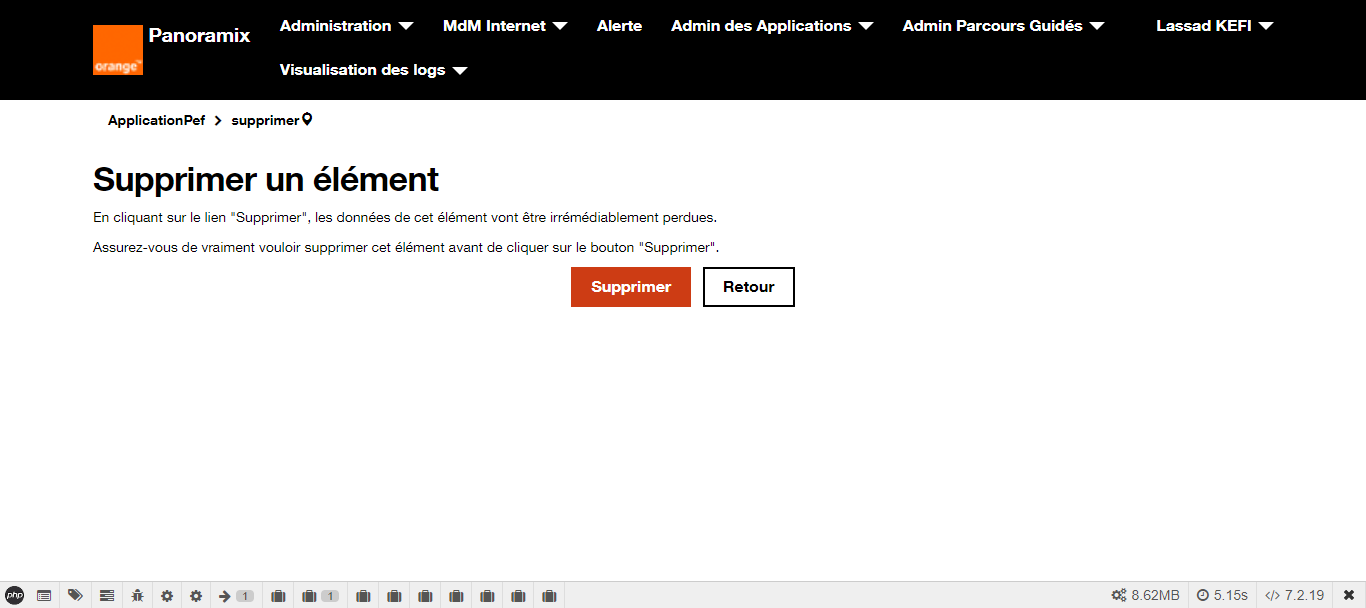
\includegraphics[width=0.7\linewidth]{img/screenshots/pef/delete}
		\caption[Interface supprimer un PEF]{Interface supprimer un PEF}
		\label{fig:delete-pef}
	\end{figure}
\end{itemize}
\newpage
\subsection{Interfaces de consultation des types de PEF}
\begin{itemize}
	\item Consultation des types de PEF et recherche
	\begin{figure}[H]
		\centering
		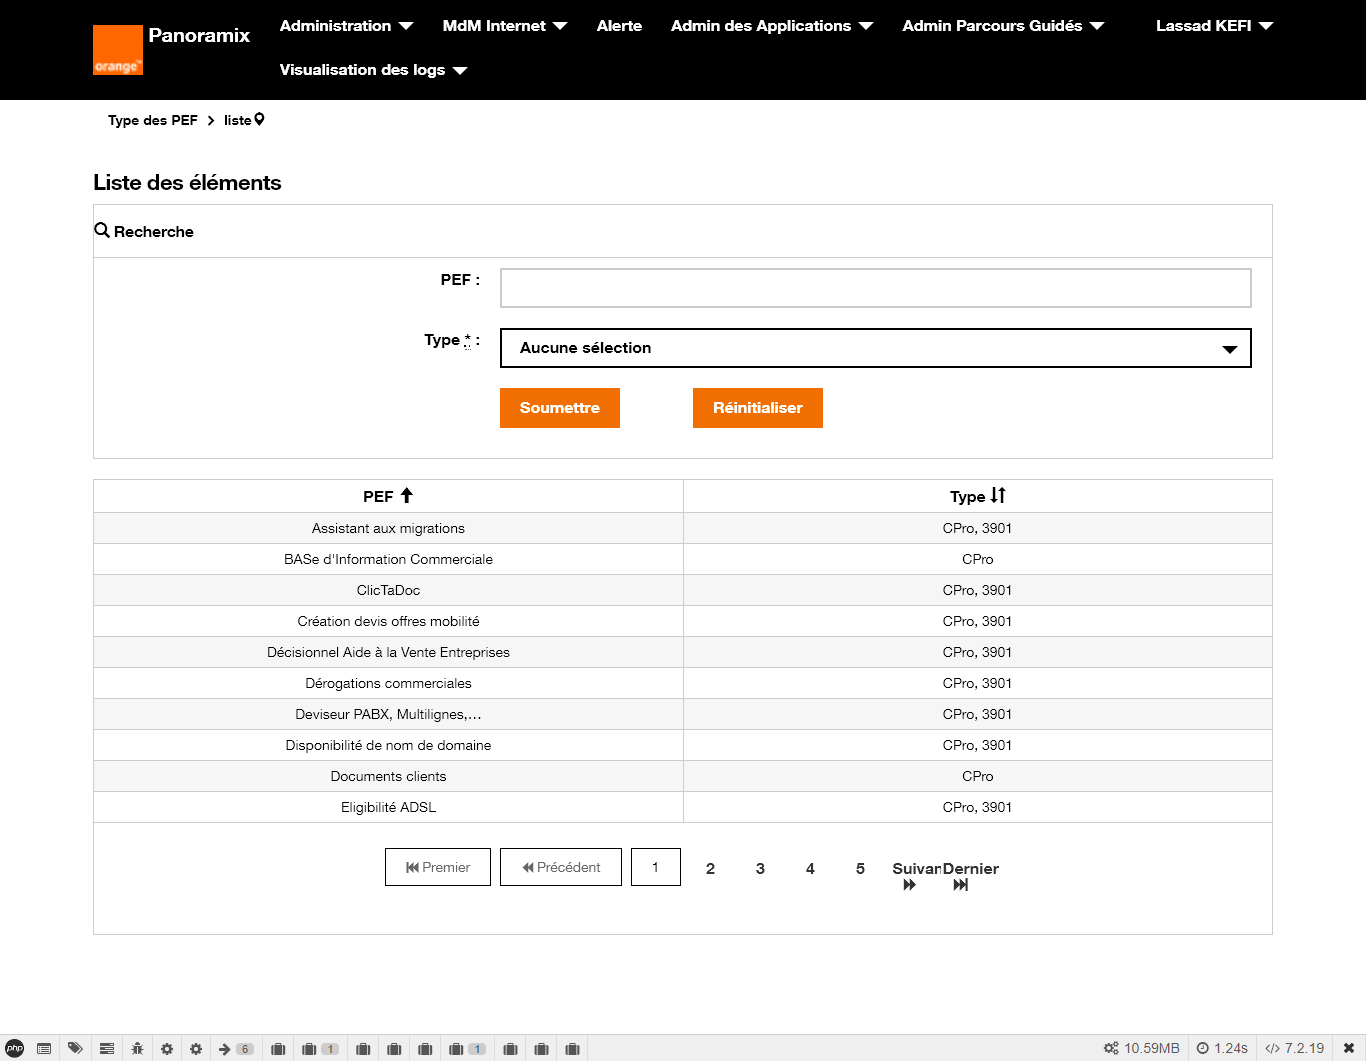
\includegraphics[width=0.7\linewidth]{img/screenshots/pef-type/index}
		\caption[Interface consultation des types de PEF et recherche]{Interface consultation des types de PEF et recherche}
		\label{fig:index-tp}
	\end{figure}
	
	\item Voir un type de PEF 
	\begin{figure}[H]
		\centering
		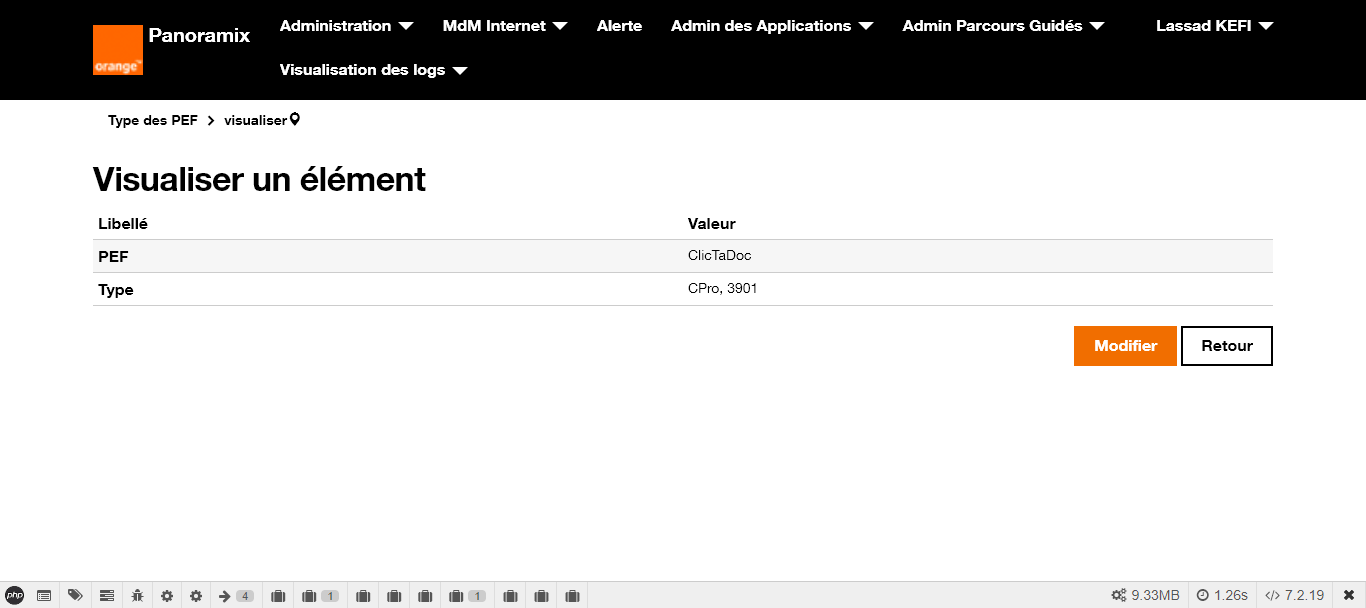
\includegraphics[width=0.7\linewidth]{img/screenshots/pef-type/view}
		\caption[Interface voir un type de PEF ]{Interface voir un type de PEF }
		\label{fig:view-tp}
	\end{figure}
\end{itemize}
\newpage
\subsection{Interfaces de visibilité des PEF aux boutiques}
\begin{itemize}
	\item Consultation des visibilités et recherche
	\begin{figure}[H]
		\centering
		\includegraphics[width=0.7\linewidth]{"img/screenshots/visibilité pef-boutique/index"}
		\caption[Interface consultation des visibilités et recherche]{Interface consultation des visibilités et recherche}
		\label{fig:index-visib}
	\end{figure}
	
	\item Voir une visibilité 
	\begin{figure}[H]
		\centering
		\includegraphics[width=0.7\linewidth]{"img/screenshots/visibilité pef-boutique/view"}
		\caption[Interface voir une visibilité]{Interface voir une visibilité }
		\label{fig:view-visib}
	\end{figure}

	\item Modifier ou créer une visibilité 
	\begin{figure}[H]
		\centering
		\includegraphics[width=0.7\linewidth]{"img/screenshots/visibilité pef-boutique/view"}
		\caption[Interface modifier ou créer une visibilité]{Interface modifier ou créer une visibilité}
		\label{fig:edit-visib}
	\end{figure}

	\item Supprimer une visibilité 
	\begin{figure}[H]
		\centering
		\includegraphics[width=0.7\linewidth]{"img/screenshots/visibilité pef-boutique/view"}
		\caption[Interface supprimer une visibilité]{Interface supprimer une visibilité}
		\label{fig:delete-visib}
	\end{figure}
	
\end{itemize}
\subsection{Interfaces de consultation des PEF au fiche client}
\begin{figure}[H]
	\centering
	\includegraphics[width=0.7\linewidth]{"img/screenshots/fiche client/fiche client et accès au pef"}
	\caption[Interface de consultation des PEF au fiche client]{Interface de consultation des PEF au fiche client}
	\label{fig:fiche-client-et-acces-au-pef}
\end{figure}

\subsection{Interface de consultation des log API}
\begin{figure}[H]
	\centering
	\includegraphics[width=0.7\linewidth]{"img/screenshots/logs + srcd/detailed log"}
	\caption[Interface de consultation des log API]{Interface de consultation des log API}
	\label{fig:detailed-log}
\end{figure}

\subsection{Capture de fichier de logs d’application Panoramix}

\begin{figure}[H]
	\centering
	\includegraphics[width=1\linewidth]{"img/screenshots/logs + srcd/log-application"}
	\caption[Capture de fichier de logs d’application Panoramix]{Capture de fichier de logs d’application Panoramix}
	\label{fig:log-application}
\end{figure}

\section*{Conclusion}
Dans ce chapitre, nous avons terminé le dernier sprint de notre application Panoramix et donc nous avons terminé le dernier release en traitant les détails de la réalisation de notre sprint et en montrant les différentes interfaces de notre application.






